\documentclass[11pt]{article}
%%% Preamble for Pomona Linguistics Paper Template %%%

%%%%%%%%%%%%%%%%%%%%%%%%%%%%
%% Document Setup & Layout
%%%%%%%%%%%%%%%%%%%%%%%%%%%%
\usepackage[utf8]{inputenc}
\usepackage[margin=1in]{geometry}
\usepackage{titlesec}
\usepackage[parfill]{parskip}
\setlength{\parindent}{20pt}
\usepackage{setspace}
\singlespacing %\doublespacing 
\sloppy
%%%%%%%%%%%%%%%%%%%%%%%%%%%%
%% Math & Logic
%%%%%%%%%%%%%%%%%%%%%%%%%%%%

\usepackage{amsmath, amssymb, amsfonts, amsthm}
\usepackage{pifont}
\newcommand{\cmark}{\ding{51}}%
\newcommand{\xmark}{\ding{55}}%
\theoremstyle{definition}
\newtheorem{definition}{Definition}[section]
\newcommand{\kuo}[1]{(\ref{#1})}
\newcommand{\forth}[1]{(\citeauthor{#1} (forthcoming)}
\usepackage{expex}

%%%%%%%%%%%%%%%%%%%%%%%%%%%%
%% Fonts & Symbols
%%%%%%%%%%%%%%%%%%%%%%%%%%%%

%\usepackage{fourier}
\usepackage{libertine}
\usepackage{tipa}         % For IPA symbols
\usepackage{textgreek}    % Greek outside math mode
\usepackage{ulem}         % Underline/strikeout


%%%%%%%%%%%%%%%%%%%%%%%%%%%%
%% Tables & Figures
%%%%%%%%%%%%%%%%%%%%%%%%%%%%

\usepackage{booktabs, caption, makecell, array, tabularx, multirow, multicol}
\usepackage{adjustbox}
\usepackage{float}
\usepackage{graphicx}
\usepackage{subcaption}
\usepackage[table]{xcolor}




%%%%%%%%%%%%%%%%%%%%%%%%%%%%
%% Trees & Diagrams
%%%%%%%%%%%%%%%%%%%%%%%%%%%%
\usepackage[linguistics]{forest}
%\forestset{
%  asr/.style={
%    for tree={
%      align=center,
%      parent anchor=south,
%      s sep=4mm,
%      l sep=6mm
%    }
%  },
%  strike/.style={
%    edge label={
%      node[midway, sloped, rotate=90] {=}
%    }
%  }
%}
\usepackage{qtree}

% Arrows and positioning
\usepackage{tikz}
\usetikzlibrary{arrows, arrows.meta, positioning, matrix, tikzmark}
\usepackage{pstricks, pst-node}

% TikZ node circle command
\newcommand{\circled}[1]{\begin{tikzpicture}[baseline=(word.base)]
\node[draw, rounded corners, text height=8pt, text depth=2pt, inner sep=2pt,
outer sep=0pt, use as bounding box] (word) {#1};
\end{tikzpicture}
}
\tikzset{state/.style={circle, draw, minimum size=20pt, inner sep=5pt}}

%%%%%%%%%%%%%%%%%%%%%%%%%%%%
%% Algorithms
%%%%%%%%%%%%%%%%%%%%%%%%%%%%

\usepackage{algorithm}
\usepackage{algpseudocode}
\algrenewcommand\algorithmiccomment[1]{\hfill{\footnotesize\textit{// #1}}}
%\algrenewcommand\algorithmiccomment[1]{\hfill$\triangleright$~
%{\footnotesize\textit{#1}}}


%%%%%%%%%%%%%%%%%%%%%%%%%%%%
%% Linguistics & Glossing
%%%%%%%%%%%%%%%%%%%%%%%%%%%%

\usepackage{leipzig}
\usepackage{expex}
\usepackage{gb4e}
\noautomath % needed for gb4e in some cases
\usepackage{phonrule} % SPE-style rules
\usepackage{marvosym}
%%%%%%%%%%%%%%%%%%%%%%%%%%%%
%% Text & Misc
%%%%%%%%%%%%%%%%%%%%%%%%%%%%

\usepackage{enumitem}
\setlist[itemize]{itemsep=1mm, parsep=0pt}
\usepackage{ragged2e}
\usepackage{stackengine}
\usepackage{verbatim}
\usepackage{todonotes}
\usepackage{color, soul}
\usepackage{metalogo}  % for XeLaTeX logo, etc.

\usepackage{bm} % for bold math symbols
%\usepackage{wasysym}
%%%%%%%%%%%%%%%%%%%%%%%%%%%%
%% Hyperlinks & Citations
%%%%%%%%%%%%%%%%%%%%%%%%%%%%

\usepackage[
  colorlinks = true,
  linkcolor = blue,
  urlcolor  = blue,
  citecolor = blue,
  anchorcolor = blue
]{hyperref}
\usepackage{natbib}

%%%%%%%%%%%%%%%%%%%%%%%%%%%%
%% Shortcuts & Tweaks
%%%%%%%%%%%%%%%%%%%%%%%%%%%%

\usepackage{xspace}
\xspaceaddexceptions{]\}}

% Replace default emptyset with nicer one

\makeatletter
\def\maketitle{%
  \begin{center}
    {\Large \bfseries \color{black} \@title \par}

%    {\normalsize \@author \par}

%    {\small \@date \par}
  \end{center}
}
\makeatother

\let\oldemptyset\emptyset
\let\emptyset\varnothing
\newcommand{\nothing}{$\emptyset$}

% Leipzig glossing again (required by some documents)
\RequirePackage{leipzig}

%%%%%%%%%%%%%%%%%%%%%%%%%%%%%%%%%%%%%%%%%%%%%%%%
%% END of preamble
%%%%%%%%%%%%%%%%%%%%%%%%%%%%%%%%%%%%%%%%%%%%%%%%

\title{Register and Representation of Shanghai Chinese}
\begin{document}
\maketitle

Shanghainese (Shanghai Chinese) is a variety of Wu Chinese spoken in Shanghai. 
It has long served as an important case for illustrating the interaction 
between tone and segmental features. Despite being relatively well studied, 
Shanghainese still presents a number of long-standing, unresolved debates 
concerning the behavior and representation of its tones. One of the central 
debates concerns the representation of register. 
\citet{yip1980}. Murmur is a phonetic manifestation of register: in addition to 
the usual pitch lowering, it is accompanied by breathy voice. Previous research 
differs on where register should be located within tonal geometry. Two 
competing views exist: one treats register as a feature that dominates at the 
word level, while the other treats it as a feature associated with the voicing 
node of a segment.

This paper is motivated by that question and has two goals. First, we provide a 
more rigorous mathematical framework to model these two approaches, allowing 
for a precise comparison of their predictive power and expressiveness. 
Second, we employ computational methods to learn the tonotactics of 
Shanghainese under both representational assumptions, comparing the learning 
results to evaluate their relative outcomes.


\section{Shanghai Tonology}

Shanghai Chinese has five tones (T1–T5). Previous research has shown a variety 
of transcription systems for these tones, whether using the five-point scale 
notation \citep{chao1930system} or more phonologically oriented representations 
indicating tonal height \citep{yip1980}. These systems largely converge on the 
overall contour shapes but differ in the precise pitch value of tonal onsets 
and offsets. 

\begin{table}[htbp]
	\centering
	\begin{tabular}{cccccc}
		\toprule
		Tone & \citet{MFCdatabase} & \citet{xu1988description} & \citet{duanmu1999metrical} &  ?  & \citet{zee1979tones} \\ \midrule
		 T1  &         53          &            53             &            /HL/            & /H/ &          HL          \\
		 T2  &         34          &            24             &            /LH/            & /L/ &         /MM/         \\
		 T3  &         23          &            13             &            /LH/            & /L/ &         /ML/         \\
		 T4  &          5          &         \emph{55}         &            /LH/            & /L/ &         /H/          \\
		 T5  &         12          &         \emph{13}         &            /LH/            & /L/ &         /LM/         \\ \bottomrule
	\end{tabular}
	\caption{Transcriptions of Shanghai tones across sources}
	\label{tab:transcript}
\end{table}


The Shanghai tonal system is regarded as a \textit{complex} system. Unlike 
Mandarin, in which tonal contrasts are primarily distinguished by pitch, tonal 
recognition in Shanghai Chinese also relies on \textit{register }and vowel 
\textit{length} \citep{zhu+2015tone}. As shown in Figure~\ref{tab:shanghai}, 
there are two registers \textsc{[upper]} (discussed in detail in the next 
section), and two major syllable types: slack syllables and checked syllables 
(those closed by a glottal stop). The following section will focus on previous 
studies of register and length contrasts in Shanghai tonology.

\begin{table}[h!]
	\centering
	\begin{tabular}{ccccccccc}
		\toprule
		\multirow{2}{*}{\textbf{Register}} & \multirow{2}{*}{\textbf{Tone}} 
		& \multicolumn{3}{c}{Slack syllable} & & \multicolumn{3}{c}{Checked syllable} \\ 
		\cmidrule{3-5}\cmidrule{7-9}
		&  & \textbf{TV(\ng)} & \textbf{DV(\ng)} & \textbf{SV(\ng)} & & \textbf{TV\textglotstop} & \textbf{DV\textglotstop} & \textbf{SV\textglotstop} \\
		\midrule
		\multirow{3}{*}{\textbf{+upper}} 
		& \textbf{T1} & pa ``father'' & \texttimes & ma ``mother'' & & \texttimes & \texttimes & \texttimes \\
		& \textbf{T2} & pa ``dam''    & \texttimes & me ``pretty'' & & \texttimes & \texttimes & \texttimes \\
		& \textbf{T4} & \texttimes & \texttimes & \texttimes & & paʔ ``eight'' & \texttimes & aʔ ``duck'' \\
		\midrule
		\multirow{2}{*}{\textbf{-upper}} 
		& \textbf{T3} & \texttimes & ba ``climb'' & ma ``horse'' & & \texttimes & \texttimes & \texttimes \\
		& \textbf{T5} & \texttimes & \texttimes & \texttimes & & \texttimes & baʔ ``white'' & maʔ ``pulse'' \\
		\bottomrule
	\end{tabular}
	\caption{Co-occurrence restrictions on tones with consonants \citep{chen2015shanghai}.}
	\label{tab:shanghai}
\end{table}
\subsection{Register}
Register is the primary distinction in Shanghai tones. Although it is often 
associated with overall pitch shift cross-linguistically, in Shanghainese, a 
lower register is also accompanied by breathy phonation. \citet{yip1980} 
classifies Shanghai syllables into murmured and clear (or plain) types, with 
murmured syllables corresponding to those that co-occur with the [–upper] 
register. Murmur can thus be 
understood as the phonetic realization of Shanghai register 
\citep{zhu1999shanghai}. The terminology for this feature varies across 
researchers, including [slack] \citep{duanmu1999metrical}, [+voice] (Ren, ???), 
and [spread glottis] (Keating, as cited in \citealt{yip1993tonal}). For 
consistency, this paper will use the term register, with the understanding that 
it refers not only to pitch lowering but also to breathy phonation.

Figure~\ref{tab:shanghai} shows that all syllables with voiced obstruents 
onsets fall neatly under the [–upper] register. This is why register is often 
regarded as a feature of voicing. For syllables beginning with sonorants, 
however, both registers are possible and contrast with each other. Two points 
should be noted in the phonetic realization of register. First, in monosyllabic 
words, the [–upper] register, even when restricted to voiced obstruents, causes 
devoicing of these segments (e.g., [d] $\rightarrow$ [d̥]), nearly neutralizing 
the VOT distinction between voiced and voiceless unaspirated stops. This 
distinction is retained when the syllable occurs in a non-initial position. 
Second, in polysyllabic words, only the register of the initial syllable is 
realized on the surface, and will also dominate the whole phrase and change the 
voicing of the following consonants\todo{give some examples}.

\subsection{Representation of Shanghai Tones}
Since the register is a major distinction in shanghai tonology, many models of 
shanghai tones have been proposed based on feature geometry 
\citep{sagey1986feature}, where the most detbaitng come from where
the resgiter should locate. 

\citet{yip1993tonal} propose three possible candidates for the representation 
of register: (i) a laryngeal feature \textsc{[voice, +spread glottis]}, (ii) a 
tonal feature \textsc{[-upper]}, or (iii) a feature that has affinities with 
both tonal and laryngeal nodes. Each option has consequences. (i) directly 
predicts that murmur correlates with onset voicing, but fails to explain the 
deletion of murmur in non-initial syllables. This gap is addressed by (ii), 
which can capture murmur deletion, but does not explain why [+upper] should 
condition onset voicing. In light of this, Yip proposes that murmur should be 
analyzed as a hybrid feature, sharing properties of both laryngeal and tonal 
domains. This view, however, is challenged by \citet{zhu1999shanghai}, who 
observes that syllable-initial voiced obstruents are sometimes realized as 
voiceless (see also \citet{chen2015shanghai}).

Building on Bao’s model, Duanmu proposes that register is consistently reflected in voice quality but not always in pitch. His model treats pitch and register as two planes: one plane encodes the stiff/slack distinction in voice quality, while the other contains tonal features. Similarly, Ren (1992) treats murmur as a feature associated with the initial consonant.

Another issue in the feature geometry of Shanghainese concerns the representation of medial and coda positions. Beyond the placement of register, scholars also debate how the syllable should be internally structured. Duanmu proposes that all Chinese dialects share the same underlying syllable structure. Rather than mora theory, he employs X-slots, positing three slots under the syllable node: one for the onset and two for the rime. Zhu, however, diverges from this proposal, offering a different analysis of syllable structure in Shanghainese.



\begin{figure}[h!]
	\centering
	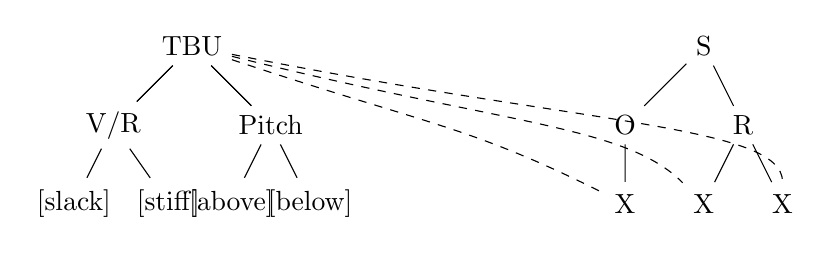
\begin{tikzpicture}[-,shorten >=1pt]
		\tikzstyle{state}=[fill=white,draw=black,text=black,node distance=16mm]
		
		% First graph (on the left)
		\node (tbu) at (1.5,0) {TBU};
		\node (R) at (.5,-1) {V/R};
		\node (P) at (2.5,-1) {Pitch};
		\node (r1) at (0,-2) {[slack]};
		\node (r2) at (1.2,-2) {[stiff]};
		\node (p1) at (2,-2) {[above]};
		\node (p2) at (3,-2) {[below]};
		\draw (tbu) -> (R) -> (r1);
		\draw (tbu) -> (R) -> (r2);
		\draw (tbu) -> (P) -> (p1);
		\draw (tbu) -> (P) -> (p2);
		
		
		% Second graph (shifted right)
		\begin{scope}[xshift=8cm]
			\node (sS) at (0,0) {S};
			\node (o) at (-1,-1) {O};
			\node (r) at (0.5,-1) {R};
			\node (x1) at (-1,-2) {X};
			\node (x2) at (0,-2) {X};
			\node (x3) at (1,-2) {X};
			\draw (sS) -> (o) -> (x1);
			\draw (sS) -> (r) -> (x2);
			\draw (r) -> (x3);
		\end{scope}
		
		% Cross edges from TBU to Xs
		\draw[dashed] (tbu) .. controls +(3,-1) and +(-2,1) .. (x1);
		\draw[dashed] (tbu) .. controls +(4,-1) and +(-1,1) .. (x2);
		\draw[dashed] (tbu) .. controls +(5,-1) and +(0,1) .. (x3);
		
	\end{tikzpicture}
\end{figure}

\begin{figure}[h!]
	\centering
	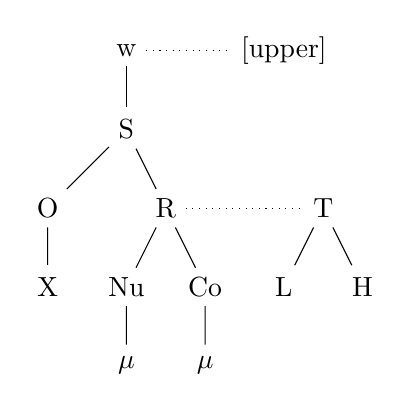
\begin{tikzpicture}[-,shorten >=1pt]
		\tikzstyle{state}=[fill=white,draw=black,text=black,node distance=16mm]
		
		\node (w) at (0,1) {w};
		\node (re) at (2,1) {[upper]};
		\node (s) at (0,0) {S};
		\node (o) at (-1,-1) {O};
		\node (r) at (0.5,-1) {R};
		\node (T) at (2.5,-1) {T};
		\node (t1) at (2.0,-2) {L};
		\node (t2) at (3,-2) {H};
		
		\node (x1) at (-1,-2) {X};
		\node (x2) at (0,-2) {Nu};
		\node (x3) at (1,-2) {Co};
		\node (m1) at (0,-3) {$\mu$};
		\node (m2) at (1,-3) {$\mu$};
		\draw (w) -> (s);
		\draw (T) -> (t1);
		\draw (T) -> (t2);
		\draw (s) -> (o) -> (x1) ;
		\draw (s) -> (r) -> (x2) -> (m1);
		\draw (r) -> (x3) -> (m2);
		\draw [dotted](r) -> (T);
		\draw [dotted](w) -> (re);
	\end{tikzpicture}
\end{figure}



\bibliography{refs.bib}
\bibliographystyle{apalike}
\end{document}